\begin{enumerate}
	\item Exercício
	
	\begin{figure}[htb]
		\caption{Integrais duplas - Aula 3 - Exercício I}
		\label{v03_a03_e01}
		\centering
		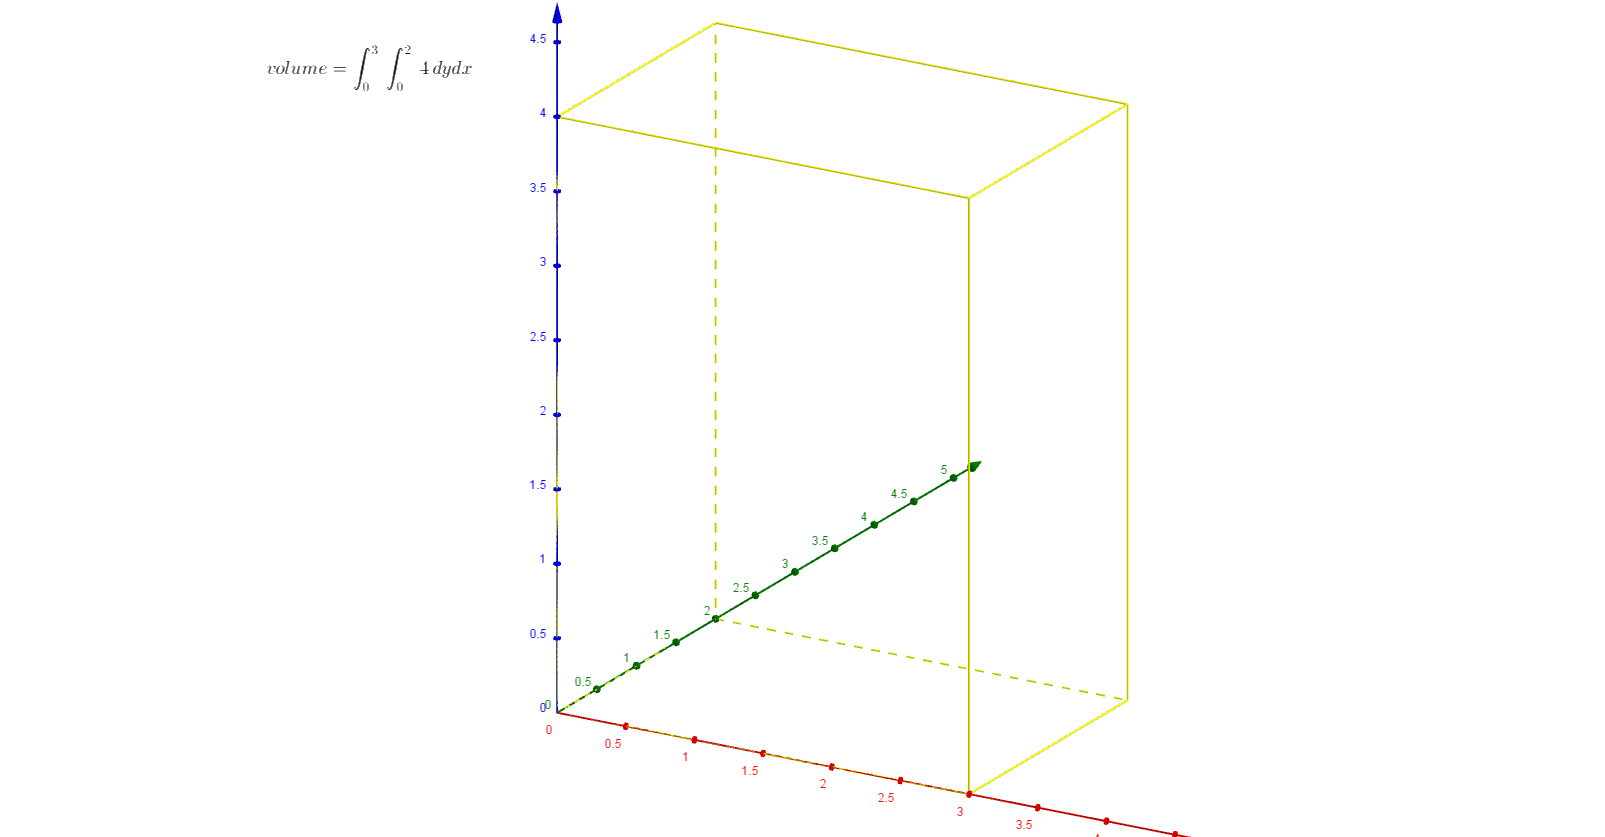
\includegraphics[width=0.5\textwidth]{v03_a03_e01.png}		
	\end{figure}
	
	\begin{equation*}
		z = 4;\; dz = dx dy	
	\end{equation*}	
	\begin{align*}
		v = \int_0^3 \int_0^2 z\, dz = \int_0^3 \int_0^2 4\, dy dx = 4\int_0^3 dx \int_0^2 dy = 4\int_0^3 dx\, [y]_0^2 = 4\int_0^3 dx\, [2 - 0] =\\ 8\int_0^3 dx = 8[x]_0^3 = 8[3 - 0] = 8 \cdot 3 = 24
	\end{align*}
		
	\item Exercício
	\begin{equation*}
		R = [0, 3] \times [0,4]
	\end{equation*}
	\begin{equation*}
		\iint_R (8 - 2y) da
	\end{equation*}
	
	\begin{figure}[htb]
		\caption{Integrais duplas - Aula 3 - Exercício II}
		\label{v03_a03_e02}
		\centering
		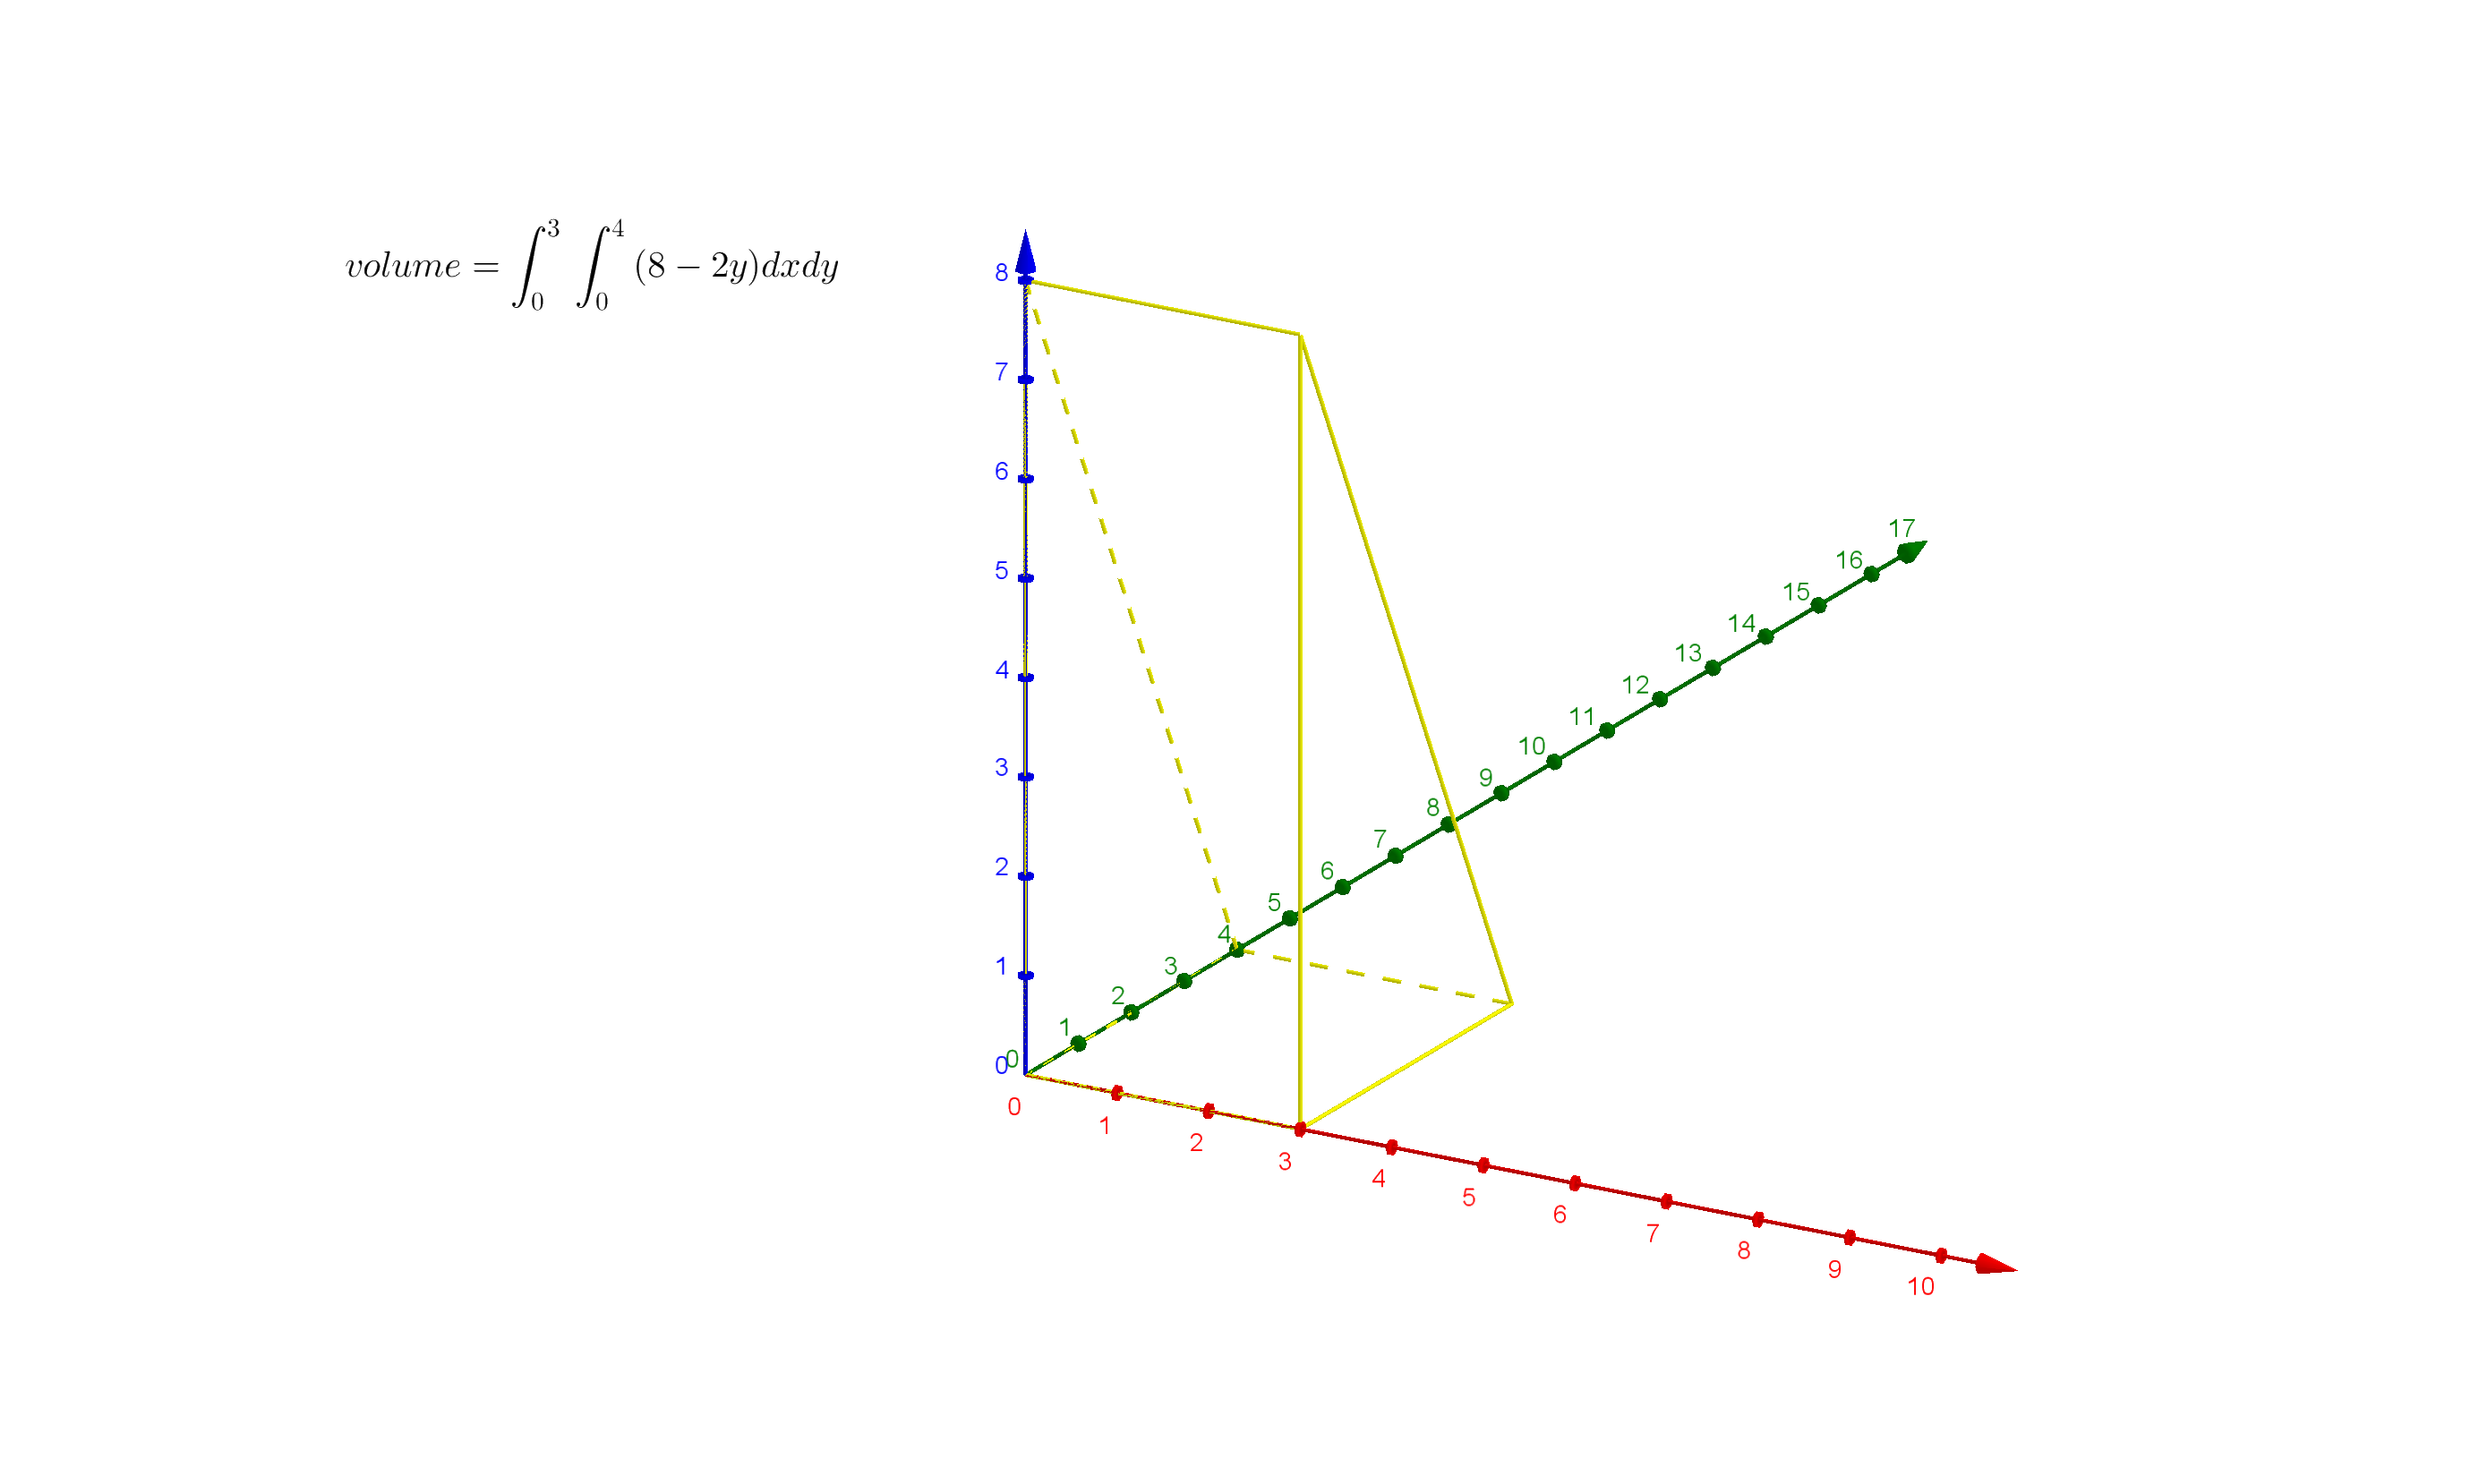
\includegraphics[width=0.5\textwidth]{v03_a03_e02.png}		
	\end{figure}	
	
	\begin{equation*}
		z = 8 - 2y;\; da = dz = dx dy
	\end{equation*}
	\begin{align*}
		v = \int_0^3 \int_0^4 z\,dz = \int_0^3 \int_0^4(8 - 2y)dx dy = \int_0^3 dx \int_0^4(8 - 2y) dy =\\ \int_0^3 dx \left(8\int_0^4 dy - 2\int_0^4 y\,dy\right) = \int_0^3 dx\, 2\left(4\int_0^4 dy - \int_0^4 y\,dy\right) =\\ 2\int_0^3 dx \left[4y - \dfrac{y^2}{2}\right]_0^4 = 2\int_0^3 dx \left[\dfrac{8y - y^2}{2}\right]_0^4 = \overstrike{2}\int_0^3 dx\, \dfrac{1}{\overstrike{2}}[y(8 - y)]_0^4 =\\ \int_0^3 dx[4(8 - 4) \overstrike{- 0(8 - 0)}] = 16\int_0^3 dx = 16[x]_0^3 = 16[3 - 0] = 48
	\end{align*}
\end{enumerate}